\documentclass[10pt, leqno]{amsart}

\usepackage{algorithm}
\usepackage[noend]{algpseudocode}
\usepackage{amsfonts}
\usepackage{amsmath}
\usepackage{amssymb}
\usepackage{amsthm}
\usepackage[backend=biber, citestyle=numeric-comp, bibstyle=ieee]{biblatex}
\usepackage{changepage}
\usepackage{enumitem}
\usepackage{fancyhdr}
\usepackage{fontspec}
\usepackage{fullpage}
\usepackage[hidelinks]{hyperref}
\usepackage{marvosym}
\usepackage{mathtools}
\usepackage[]{mdframed}
\usepackage{physics}
\usepackage[skins]{tcolorbox}
\usepackage{thmtools}

\usepackage{tikz-3dplot}
\usetikzlibrary{angles, calc, cd, quantikz, quotes, patterns}
\usepackage{titlesec}
\usepackage{wasysym}

\usepackage{tikz-cd}

\usepackage{bookmark}
\usepackage[nameinlink]{cleveref}

\titleformat{\section}[runin]{\normalsize\bfseries}{\thesection}{1em}{}[]
\titleformat{\subsection}[runin]{\normalsize\bfseries}{\thesubsection}{1em}{}[]
\titleformat{\subsubsection}[runin]{\normalsize\bfseries}{\thesubsubsection}{1em}{}[]

\addbibresource{convex_analysis_subdifferentials_and_the_finite_dimensional_real_situation_notes.bib}

\theoremstyle{definition}
\newtheorem{theorem}{Theorem}[section]
\newtheorem{conjecture}{Conjecture}[section]
\newtheorem{definition}{Definition}[section]
\theoremstyle{remark}
\newtheorem{problem}[theorem]{Problem}
\newtheorem{lemma}[theorem]{Lemma}
\newtheorem{remark}[theorem]{Remark}
\newtheorem{observation}[theorem]{Observation}
\newtheorem{example}[theorem]{Example}
\newtheorem{corollary}[theorem]{Corollary}

\renewcommand{\qedsymbol}{\(\blacksquare\)}

\setlength{\parindent}{0pt}

\renewcommand{\theequation}{\thesection.\arabic{equation}}

\DeclareMathOperator{\controrot}{CR}
\DeclareMathOperator{\expectation}{E}
\DeclareMathOperator{\gf}{GF}
\DeclareMathOperator{\qft}{QFT}
\DeclareMathOperator{\rk}{rk}
\DeclareMathOperator{\defect}{def}
\DeclareMathOperator{\swapgate}{SWAP}
\DeclareMathOperator{\che}{CHE}
\DeclareMathOperator{\poly}{poly}
\DeclareMathOperator{\Span}{Span}
\DeclareMathOperator{\diag}{diag}

\newcommand{\djk}{\delta_{j, k}}
\newcommand{\tlk}{\tilde{\lambda_k}}

\newcommand{\evalat}[2]{\left.{#1}\middle|\right._{#2}}

% SOURCE: https://tex.stackexchange.com/questions/296151/double-head-and-hook-arrow
\newcommand{\hookdoubleheadrightarrow}{%
  \hookrightarrow\mathrel{\mspace{-15mu}}\rightarrow
}

\newtcolorbox{edgebox}{enhanced, colback=white, frame code={%
\draw[very thin] (frame.north west) -- ($(frame.north west) + ( 0.5, 0)$);
\draw[very thin] (frame.north west) -- ($(frame.north west) + (0, -0.5)$);
\draw[very thin] (frame.south east) -- ($(frame.south east) + (-0.5, 0)$);
\draw[very thin] (frame.south east) -- ($(frame.south east) + (0,  0.5)$);
}}

\AtEveryBibitem{%
  \clearfield{journaltitle}%
  \clearfield{date}%
  \clearfield{volume}%
  \clearfield{pages}%
  \clearfield{publisher}%
  \clearfield{number}%
  \clearfield{journaltitle}%
}

\newcommand{\commentcmd}[1]{}

%\newcommand{\draftcommenttodo}{\textcolor{red}{ TODO }}
%\newcommand{\draftcommentdone}{\textcolor{green}{ DONE }}
\newcommand{\draftcommenttodo}{}
\newcommand{\draftcommentdone}{}

\begin{document}
    \begin{mdframed}
        \textsc{Seminar on Convex Analysis} \hfill valentinpi\\
        Freie Universität Berlin \hfill 25 July, 2023\\
        Summer Term 2023
    \end{mdframed}

    \section*{Presentation Notes on: Further Properties of Subdifferentials and The Situation in \(\mathbb{R}^n\)}

    \phantom{}

    \commentcmd{
    \begin{center}
        \colorbox{green!15}{
            \begin{minipage}{0.95\linewidth}
                \centering
                
                \paragraph*{\textbf{\textcolor{red}{Remarks for the Meeting with Prof. Thomas}}}
                
                \begin{itemize}[wide]
                    \item In my functional analysis course, we have not seen what topological or locally convex topological vector spaces are and it is also not in the book, so I needed to research that in Jänich. I have used the practical definition, as the definition using seminorms is not important for this topic.
                    \item I have used some commutative diagrams, because the situation got a bit cluttered at some points.
                    \item I have written a small section for preliminaries, where I just list what I use and where I looked it up. Is that fine?
                    \item Why do we use the notation \(\langle x^*, x \rangle = x^*x\)? I have looked at some articles in the field because I was curious for how active it is, and it seems to be the standard there. Is it because of \(\langle x^*, \Lambda x \rangle = \langle \Lambda^* x^*, x \rangle\) by the definition of the adjoint?
                    \item Is there more intuition for the definition of the subgradient? It seems as though we took the difference quotient \((f(z)-f(x))/(z-x)\) and replaced the denominator by the value of the functional.
                    \item How does the definition of the subdifferential make sense if \(f(z)=f(x)=\infty\) for some \(z \in X\)? And if the functions are not proper and \(\neq \infty\), we may have the same situation for \(-\infty\). \(\Rightarrow\) Maybe focus on proper.
                    \item Why do we take the directional derivative in only one direction?
                    \item In Proposition 4 of 4.1, is \(x \in X\) generally?
                    \item Which date for presentation? \(\Rightarrow\) ?
                \end{itemize}
            \end{minipage}
        }
    \end{center}
    }

    \section{Preliminaries \draftcommentdone} \label{preliminaries} We first recall the following notions (without the relevant properties for now) from the previous talks. Most of the necessary related, technical theorems will be recited in dedicated boxes when needed.
    \begin{table}[!hbtp]
        \centering
        \begin{tabular}{l|l}
            \textbf{Topological Vector Spaces (TVS)} & \cite[pp. 30-31]{Jaenich}\\
            \textbf{Convex Sets}               & \cite[p. 45]{IoffeTihomirov}\\
            \textbf{Convex Hulls}              & \cite[p. 162]{IoffeTihomirov}\\
            \textbf{Kones} \(K, K_U\)          & \cite[p. 45, p. 162]{IoffeTihomirov}\\
            \textbf{Lower/Upper Semicontinuity} \(f(x) \geq f(x_0) - \varepsilon\) / \(f(x) \leq f(x_0) + \varepsilon\) & \cite[p. 12]{IoffeTihomirov}\\
            \textbf{Epigraphs} \(\text{epi}(f)\) & \cite[p. 45]{IoffeTihomirov}\\
            \textbf{Convex Functions} \(\text{conv}(\text{epi}(f))=\text{epi}(f)\) & \cite[p. 45]{IoffeTihomirov}\\
            \textbf{Jensens Inequality} \(f((1-\lambda)x+\lambda y) \leq (1-\lambda)f(x)+\lambda f(y)\)        & \cite[p. 167]{IoffeTihomirov}\\
            \textbf{Proper Functions} \(-\infty < f \neq \infty\) & \cite[p. 45]{IoffeTihomirov}\\
            \textbf{Effective Domain} \(\text{dom}(f)\) & \cite[p. 45]{IoffeTihomirov}\\
            \textbf{Affine Hull} \(\text{aff}(A)\) & \cite[p. 186]{IoffeTihomirov}\\
            \textbf{Relative Interior} \(\text{ri}(f)\) & \cite[p. 187]{IoffeTihomirov}\\
            \textbf{Subgradients} \(f(z) \geq f(x) + \langle x^*, z-x\rangle \, \forall \, z \in X\) & \cite[p. 46]{IoffeTihomirov}\\
            \textbf{Subdifferentials} \(\partial f(\cdot)\) & \cite[p. 46]{IoffeTihomirov}\\
            \textbf{Conjugates} \(f^*\)        & \cite[pp. 171-172]{IoffeTihomirov}\\
            \textbf{Directional Derivatives} \(f'(\cdot; \cdot)\) & \cite[p. 193]{IoffeTihomirov}
        \end{tabular}
    \end{table}
    %\begin{itemize}[wide]
    %    \item \textbf{Convex Sets:} A subset of a linear space \(X\) is called \emph{convex}, if any \emph{convex combination} \((1-\lambda)x+\lambda y\), \(\lambda \in [0, 1]\), of two points \(x, y \in X\) is contained inside of \(X\) \cite[p. 45]{IoffeTihomirov}.
    %    \item \textbf{Topological Vector Spaces:} A set equipped with both a topology and a linear structure is called a \emph{topological vector space}, if both vector addition and scalar multiplication are continuous in the topology of the space \cite[pp. 30-31]{Jaenich}.
    %    \item \textbf{Space of Bounded Linear Operators:} For normed spaces \(X\) and \(Y\), we shall denote the set of bounded linear operators as \(L(X, Y)\).
    %    \item \textbf{Locally Convex Topological Vector Spaces:} A topological vector space is called \emph{locally convex}, if any neighborhood of the zero and thus of any point contains a convex neighborhood \cite[p. 36]{Jaenich}.
    %    \item \textbf{Kones:} A set \(K \subseteq X\) of a topological vector space is called a \emph{cone}, if \(x \in K\) implies \(\lambda x \in K\) for any \(\lambda \in \mathbb{R}_{> 0}\). A subset \(U \subseteq X\) is a \emph{generator} of the kone \(K_U \coloneqq \{\lambda x \mid \lambda \in \mathbb{R}, x \in X\}\).
    %    \item \textbf{Convex Hulls:} Convex hull...
    %    \item \textbf{Convex Functions:} \(f\) is \emph{convex}, if \(f(\lambda x + (1-\lambda) y) \leq \lambda f(x) + (1-\lambda)f(y)\) for all \(\lambda \in [0, 1]\) and \(x, y \in X\).
    %    %\item \(f\) is \emph{lower/upper semicontinuous} in \(x \in X\), if \(\forall \, \varepsilon \in \mathbb{R}_{> 0} \, \exists \, x \in U \subseteq X \text{ open} \, \forall \, y \in U\colon f(y) \geq f(x) - \varepsilon \text{ or } f(y) \leq f(x) + \varepsilon\) respectively.
    %    \item \textbf{Proper Functions:} \(f\) is called \emph{proper}, if \(-\infty < f \neq \infty\).
    %    \item \textbf{Effective Domain:} The \emph{effective domain} of \(f\) is defined as \(\text{dom}(f) \coloneqq f^{-1}(\overline{\mathbb{R}} \setminus \{\infty\})\).
    %    \item \textbf{Relative Interior:} relative interior...
    %    \item \textbf{Subgradients:} A \emph{subgradient} of \(f\) at a point \(x \in X\) is a functional \(x^* \in X^*\) satisfying \(f(z)-f(x) \geq \langle x^*, z-x \rangle \, \forall \, z \in X\).
    %    \item \textbf{Subdifferentials:} The \emph{subdifferential} \(\partial f(x)\) of \(f\) at a point \(x \in X\) is defined to be the set of all subgradients at that point, so \(\partial f(x) = \{x^* \in X^* \mid x^* \text{ is a subgradient of \(f\) at \(x\)}\} \in \mathcal{P}(X^*)\).
    %    \item \textbf{Directional Derivatives:} Suppose \(|f| < \infty\) and \(x, y \in X\). The \emph{directional derivative of \(f\) at \(x\) in direction \(y\)} is defined as \(f'(x; y) \coloneqq \lim_{\lambda \downarrow 0} (f(x+\lambda y)-f(x))/\lambda\).
    %\end{itemize}
    From now on, assume that \(X\) and \(Y\) are separable locally convex topological vector spaces over \(\mathbb{R}\). We denote the space of continuous linear operators between them as \(L(X, Y)\) and the dual spaces as \(X^*, Y^*\). Recall that we equip these dual spaces with their respective weak\({}^*\) topologies, giving especially that any continuous functional in the bi-dual \(X^{**}\) and analogously \(Y^{**}\) is of form \(\hat{x}\colon X^* \to \mathbb{R}, x^* \mapsto \hat{x}(x^*) \coloneqq x^*(x)\) for an \(x \in X\) \cite[pp. 439-440]{Werner}. Let further \(n \in \mathbb{N}_{\geq 1}\) and \(f\colon X \to \overline{\mathbb{R}} = \mathbb{R} \cup \{\pm \infty\}\), where the closure of \(\mathbb{R}\) is taken in the canonical topology after extension by \(\pm \infty\). Also note the convention of expressing the subgradient as above \cite[p. 214]{Rockafellar}. To test it out one can quickly verify that \(f \in \{\pm \infty\}\) is subdifferentiable everywhere. Furthermore, note that we will not cite every theorem we use directly here, but we will give references at selected positions. Especially, we want to highlight the following characterizations, which we will use more-or-less implicitly throughout.

    \begin{theorem}[{\cite[pp. 170-171]{IoffeTihomirov}}] \label{proper_convex_continuity_boundedness_equivalence}
        Let \(f\) be proper and convex. Then the following statements are equivalent.
        \begin{enumerate}[label=(\roman*), wide]
            \item \(f\) is bounded on a neighborhood of \(x \in X\).
            \item \(f\) is continuous at \(x\).
        \end{enumerate}
    \end{theorem}

    \begin{theorem}[{\cite[pp. 193-199]{IoffeTihomirov}}] \label{convex_subdifferential_characterizations}
        Let \(f\) be convex. Then the following statements are equivalent.
        \begin{enumerate}[label=(\roman*), wide]
            \item \(x^* \in \partial f(x)\).
            \item \(f(z) \geq f(x) + \langle x^*, z-x \rangle \, \forall \, z \in X\).
            \item \(f(x)+f^*(x^*) = \langle x^*, x \rangle\)
            \item \label{convex_subdifferential_characterizations_4} \(f'(x, y) = \sup_{x^* \in \partial f(x)} \langle x^*, y \rangle \geq \langle x^*, y \rangle \, \forall \, y \in X\), i.e. \(x^* \in \partial f'(x; 0) = \partial f(x) = \text{dom}(f'(x; \cdot)^*)\), if \(f\) is additionally proper.
        \end{enumerate}
    \end{theorem}

    We may remark especially the rather surprising/fascinating statement in \Cref{convex_subdifferential_characterizations} \ref{convex_subdifferential_characterizations_4}. It can be proven by showing that \(f'(x; \cdot)\) supports precisely this set \cite[p. 192, p. 196]{IoffeTihomirov}, but is not clear from the definitions. We will also use the following fact about the directional derivative.

    \begin{theorem}[{Infimum Form \cite[pp. 194-195]{IoffeTihomirov}}]
        Let \(f\) be proper and convex. Then \(f'(x; \cdot)\) is well defined for any \(x \in \text{dom}(f)\), convex, proper and for any \(y \in X\)
        \begin{align}
            f'(x; y) = \inf_{\lambda \in \mathbb{R}_{> 0}} \frac{f(x+\lambda y)-f(x)}{\lambda}
        \end{align}
    \end{theorem}

    %\phantom{}

    %Essentially, we prove three theorems and a lemma, but more theorems are needed to build up these proofs.

    \section{A Chain Rule \draftcommentdone} Recall the chain rule from univariate differential calculus, which is of form \((f \circ g)' = g' \cdot (f' \circ g)\). Similar statements can be made for the subdifferential of a function with a concatenated continuous linear operator, as the following theorem establishes.

    \begin{theorem}[{\cite[p. 201]{IoffeTihomirov}}]
        Let \(\Lambda \in L(X, Y)\) and \(f\colon Y \to \overline{\mathbb{R}}\) be a function.
        \begin{enumerate}[label=(\roman*), wide]
            \item \label{compat_with_operator_theorem_1} For any \(x \in X\), we have
            \begin{align}
                \partial (f\Lambda)(x) \supseteq \Lambda^*\partial f(\Lambda x)
            \end{align}
            \item \label{compat_with_operator_theorem_2} If \(f\) is convex and proper on \(X\), as well as continuous at a point in \(\text{Im}(\Lambda)\), then for any \(x \in X\)
            \begin{align}
                \partial (f\Lambda)(x) = \Lambda^*\partial f(\Lambda x) \label{compat_with_operator_theorem_eq_2}
            \end{align}
        \end{enumerate}
    \end{theorem}

    \begin{figure}[!hbtp]
        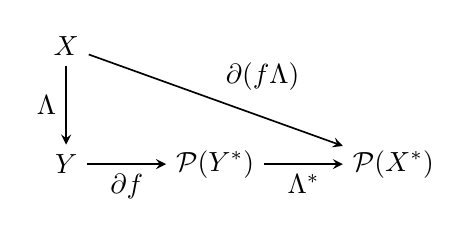
\begin{tikzpicture}[>=stealth, semithick]
            \node (0) at (0, 0) {\(X\)};
            \node[below=1cm of 0] (1) {\(Y\)};
            \node[right=1cm of 1] (2) {\(\mathcal{P}(Y^*)\)};
            \node[right=1cm of 2] (3) {\(\mathcal{P}(X^*)\)};
            \draw[->] (0) -- (1) node[left, pos=0.5] {\(\Lambda\)};
            \draw[->] (1) -- (2) node[below, pos=0.5] {\(\partial f\)};
            \draw[->] (2) -- (3) node[below, pos=0.5] {\(\Lambda^*\)};
            \draw[->] (0) -- (3) node[above right, pos=0.5] {\(\partial (f\Lambda)\)};
        \end{tikzpicture}
    \end{figure}

    \begin{proof}
        \begin{enumerate}[label=(\roman*), wide]
            \item[\ref{compat_with_operator_theorem_1}] \draftcommentdone Fix an \(x \in X\) and let \(x^* \in \Lambda^*\partial f(\Lambda x)\). Then \(\exists \; y^* \in \partial f(\Lambda x)\), s.t. \(x^* = \Lambda^* y^* = y^* \Lambda\). Then \(y^*\) fulfills by definition
            \begin{align}
                f(z') \geq f(\Lambda x) + \langle y^*, z'-\Lambda x \rangle
            \end{align}
            for any \(z' \in Y\). As \(\Im(\Lambda) \subset Y\), we may assume \(z' = \Lambda z\) for a \(z \in X\) and obtain
            \begin{align}
                (f \Lambda)(z) \geq (f \Lambda)(x) + \langle y^*, \Lambda (z - x) \rangle = (f \Lambda)(x) + \langle x^*, z - x \rangle
            \end{align}
            by the notation used.\footnote{The full calculation reads \(\langle y^*, \Lambda (z-x) \rangle = (y^* \Lambda) (z-x) = (\Lambda^* y^*) (z-x) = \langle x^*, z-x \rangle\).}
            \item[\ref{compat_with_operator_theorem_2}] \draftcommentdone If \((f\Lambda)(x) = \infty\), then \(\partial (f\Lambda)(x) = \emptyset\), giving with \ref{compat_with_operator_theorem_1} the equality. Denote now the point at which \(f\) is continuous as \(\Lambda \bar{x}\), \(\bar{x} \in X\) and additionally fix an \(x \in X\). First, we show that \(f'(\Lambda x; \cdot)\) is continuous at a point in \(\Im(\Lambda)\) \ref{compat_with_operator_theorem_2_1}. In the second step, we use a rule on interchanging conjugates with adjoints to directly obtain the statement \ref{compat_with_operator_theorem_2_2}.
            
            \begin{enumerate}[label=(\alph*), wide]
                \item \label{compat_with_operator_theorem_2_1} The argument requires the following theorem.
                
                \begin{edgebox}
                    \begin{theorem}[{\cite[pp. 195-196]{IoffeTihomirov}}] \label{point_directional_derivative_continuity_theorem}
                        Let \(f\colon X \to \overline{\mathbb{R}}\) be a proper, convex function, which is continuous on \(\emptyset \neq U \subseteq X\) and \(x \in X\) be fixed.
                        \begin{enumerate}[label=(\roman*), wide]
                            \item \label{point_directional_derivative_continuity_theorem_1} If \(|f'(x; \bar{x})| < \infty\) for \(\bar{x} \in X\) with \(x+\bar{x} \in U\), then \(f'(x; \cdot)\) is continuous on \(K_{U - \{x\}} \setminus \{0\}\)\footnote{The minus sign \(-\) here denotes the algebraic difference of sets.}.
                            \item \label{point_directional_derivative_continuity_theorem_2} If \(f\) is continuous at \(x\), then \(f'(x; \cdot)\) is finite and continuous on \(X\).
                        \end{enumerate}
                    \end{theorem}
                \end{edgebox}
    
                \begin{figure}[!hbtp]
                    \centering
                    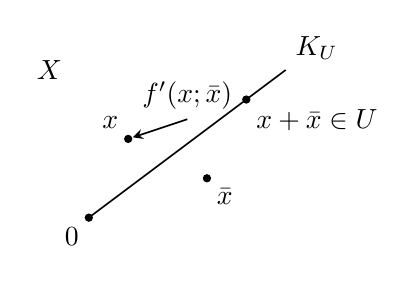
\begin{tikzpicture}[>=stealth, scale=1, semithick]
                        \tikzset{point/.style={circle, fill, inner sep=0pt, minimum size=3pt}};
                        \node[point] (0) at (0, 0) {};
                        \node[below left] at (0) {\(0\)};
                        \node[point] (x) at (0.5, 1) {};
                        \node[above left] at (x) {\(x\)};
                        \node[point] (barx) at (1.5, 0.5) {};
                        \node[below right] at (barx) {\(\bar{x}\)};
                        \draw (0, 0) -- (2.5*1, 2.5*0.75) node[above right] {\(K_U\)};
                        \node[point] (xplusbarx) at (2, 1.5) {};
                        \node[below right] at (xplusbarx) {\(x+\bar{x} \in U\)};
                        \draw[<-] (x) -- ($(x)!0.5!(xplusbarx)$) node[above] {\(f'(x; \bar{x})\)};
                        \node at (-0.5, 2.5*0.75) {\(X\)};
                    \end{tikzpicture}
                    \caption{Illustration of the situation in \Cref{point_directional_derivative_continuity_theorem}.}
                \end{figure}
                
                Consider that \(f\) is continuous in \(\{\Lambda \bar{x} = \Lambda x + \Lambda (\bar{x}-x)\}\) and use the bound
                \begin{align}
                    f'(\Lambda x; \Lambda (\bar{x}-x)) &= \lim_{\lambda \downarrow 0} \frac{f(\Lambda x + \lambda \Lambda (\bar{x}-x)) - f(\Lambda x)}{\lambda}\\
                    &\leq \lim_{\lambda \downarrow 0} \frac{(1-\lambda)f(\Lambda x) + \lambda f(\Lambda \bar{x}) - f(\Lambda x)}{\lambda} = f(\Lambda \bar{x}) - f(\Lambda x) \overset{\ref{compat_with_operator_theorem_2_1_1}}{\leadsto} |f'(\Lambda x; \Lambda (\bar{x}-x))| < \infty
                \end{align}
                \begin{enumerate}[label=(\arabic*), wide]
                    \item \label{compat_with_operator_theorem_2_1_1} Since \(f\) is convex and continuous at \(\Lambda \bar{x}\), it is finite there.
                \end{enumerate}
                By \Cref{point_directional_derivative_continuity_theorem} \ref{point_directional_derivative_continuity_theorem_1}, \(f'(\Lambda x; \cdot)\) is continuous on \(K_{\{\Lambda \bar{x}\} - \{\Lambda x\}} \setminus \{0\}\). If \(\bar{x} \neq x\), then we are done. Otherwise, as \(f\) is continuous at \(\Lambda x\), thus by \Cref{point_directional_derivative_continuity_theorem} \ref{point_directional_derivative_continuity_theorem_2}, \(f'(\Lambda x; \cdot)\) is continuous everywhere, especially at a point of \(\Im(\Lambda)\).
                \item \label{compat_with_operator_theorem_2_2} Consider first the following adjoint rule.

                \begin{edgebox}
                    \begin{theorem}[{\cite[p. 179, p. 183]{IoffeTihomirov}}] \label{adjoint_calculation_rule}
                        Let \(\Lambda \in L(X, Y)\) and \(f\colon Y \to \overline{\mathbb{R}}\) be a convex function, continuous at a point in \(\Im(\Lambda)\). Then \((f\Lambda)^* = \Lambda^* f^*\) and for each \(x^* \in \text{dom}((f\Lambda)^*)\), there is a \(y^* \in Y^*\) with \(x^* = \Lambda^*y^*\) and \((f\Lambda)^*(x^*) = f^*(y^*)\).
                    \end{theorem}
                \end{edgebox}
    
                The statement is now given by the following calculation.
                \begin{align}
                    \partial (f\Lambda)(x) \overset{\ref{compat_with_operator_theorem_2_2_1}}{=} \partial (f'(\Lambda x; \cdot)\Lambda)(0) \overset{\ref{compat_with_operator_theorem_2_2_2}}{=} \Lambda^* \partial f'(\Lambda x; 0) = \Lambda^* \partial f(\Lambda x)
                \end{align}
                \begin{enumerate}[label=(\arabic*), wide]
                    \item \label{compat_with_operator_theorem_2_2_1} Recall the equivalent definition \(\partial (f\Lambda)(x) = \partial (f\Lambda)'(x; 0) = \{x^* \in X^* \mid (f\Lambda)'(x; y) \geq \langle x^*, y\rangle \, \forall \, y \in X\}\) for subdifferentials at a point. Then use the fact that \((f\Lambda)'(x; z) = f'(\Lambda x; \Lambda z)\) for \(x, z \in X\) by
                    \begin{align}
                        (f\Lambda)'(x; z) &= \lim_{\lambda \downarrow 0} \lambda^{-1} ((f\Lambda)(x + \lambda z) - (f\Lambda)(x)) = \lim_{\lambda \downarrow 0} \lambda^{-1} (f(\Lambda x + \lambda \Lambda z) - f(\Lambda x)) = f'(\Lambda x; \Lambda z)
                    \end{align}
                    \item \label{compat_with_operator_theorem_2_2_2} We show both directions of the set equality.
                    \begin{itemize}[wide]
                        \item[\((\subseteq)\)] Recall that \(f'(\Lambda x; \cdot)\) is convex, and that \(x^* \in \partial (f'(\Lambda x; \cdot) \Lambda)(0)\) means \(x^* \in \text{dom}((f'(\Lambda x; \cdot)\Lambda)^*)\). Applying \Cref{adjoint_calculation_rule} then gives a \(y^* \in Y^*\) with \(x^* = \Lambda^* y^*\) and \((f'(\Lambda x; \cdot)\Lambda)^*(x^*)=f'(\Lambda x; \cdot)^*(y^*)\). For the direction, it suffices to prove that \(y^* \in \partial f'(\Lambda x; 0) = \partial f(\Lambda x)\). By the characterization of subgradients for convex functions, it further suffices to prove \(f'(\Lambda x; \Lambda x) + (f'(\Lambda x; \cdot))^*(y^*) = \langle y^*, \Lambda x \rangle\). But we have
                        \begin{align}
                            \langle y^*, \Lambda x \rangle = \langle x^*, x \rangle = f'(\Lambda x; \Lambda x) + (f'(\Lambda x; \cdot)\Lambda)^*(x^*) = f'(\Lambda x; \Lambda x) + f'(\Lambda x; \cdot)^*(y^*)
                        \end{align}
                        Reversing the steps then gives the argument.
                        \item[\((\supseteq)\)] Let \(\Lambda^*y^* \in \Lambda^*\partial f'(\Lambda x; 0)\) for a \(y^* \in Y^*\) and let \(x' \in X\) be arbitrary. Then we have
                        \begin{align}
                            (f'(\Lambda x; \cdot)\Lambda)(x') = f'(\Lambda x; \Lambda x') \geq \langle y^*, \Lambda x' \rangle = \langle \Lambda^* y^*, x' \rangle
                        \end{align}
                        so \(\Lambda^* y^* \in \partial (f'(\Lambda x; \cdot) \Lambda) (0)\).
                    \end{itemize}
                \end{enumerate}
            \end{enumerate}
        \end{enumerate}
    \end{proof}

    \begin{remark}
        Note that the statement from \cite[p. 201]{IoffeTihomirov} misses the fact that \(f\) needs to at least be proper. If \(f\) is not proper, i.e. \(-\infty \in \Im(f)\) or \(f = \infty\), and assuming that we have defined the subdifferential analogously for arbitrary functions of form \(X \to \overline{\mathbb{R}}\), then we can distinguish three cases.
        \begin{enumerate}[label=(\roman*), wide]
            \item \label{chain_rule_remark_1} Suppose \(f = -\infty\). Then \(\partial (f\Lambda)(x) = X^*\), but \(\Lambda^* \partial f(\Lambda x) = \Im(\Lambda^*)\). Unless \(\Lambda^*\) is an epimorphism, the equality does not hold.
            \item Now suppose \(-\infty \in \Im(f)\) and that there is a point \(x' \in X\) with \(f(x') > -\infty\). Then \(\partial f(x') = \emptyset\) and \(\partial f(x_{-\infty}) = X^*\) generally for any \(x_{-\infty} \in f^{-1}(\{-\infty\})\). Note that we let \(x'\) and \(x_{-\infty}\) be loose. We shall skip a full characterization of this case depending on \(\Im(\Lambda)\) here.
            \item For \(f = \infty\), we apply the same argument as in \ref{chain_rule_remark_1}.
        \end{enumerate}
    \end{remark}

    %\begin{example}
    %    We demonstrate the chain rule on a small example. Let \(X = \mathbb{R}\) and set \(f\colon \mathbb{R} \to \mathbb{R}, x \mapsto x^{2m}\) for some \(m \in \mathbb{N}_{\geq 0}\). Furthermore, for a fixed \(x \in \mathbb{R}\), let \(\Lambda \in L(\mathbb{R}, \mathbb{R})\) be given by \(z \mapsto z - x\). Then \(\Lambda(x) = 0\). We want to compute the subdifferential \(\partial (f\Lambda)(x)\). We have
    %    \begin{align}
    %        \partial f(0) = \{z \mapsto az \mid a \in \mathbb{R}, z^{2m} \geq az \, \forall \, z \in \mathbb{R}\} = \{0\}
    %    \end{align}
    %    Thus \(\partial (f\Lambda)(x) = \Lambda^* \partial f(0) = \{0\}\). % The moral of the story is, that even degree polynomials do not admit to a nonconstant subdifferential by chaining with a continuous linear operator.
    %\end{example}

    %\begin{remark}
    %    If \(\Lambda\) is bijective, then the equality in \Cref{compat_with_operator_theorem_eq_2} holds aswell.
    %\end{remark}

    \section{Supremum Functions \draftcommentdone}

    We look at descriptions of the subderivative of a supremum function over a family of convex functions.

    \begin{lemma} \label{supremum_convexity_lemma}
        Let \(\{f_s\colon X \to \overline{\mathbb{R}}\}_{s \in S}\), with \(S\) an index set, be a family of convex functions and \(\hat{f}\colon X \to \overline{\mathbb{R}}, x \mapsto \sup_{s \in S} f(x)\). Then \(\hat{f}\) is convex.
    \end{lemma}

    \begin{proof}
        \draftcommentdone Consider
        \begin{align}
            \text{epi}(\hat{f}) &= \left\{(\alpha, x) \in \mathbb{R} \times X \mid \alpha \geq \hat{f}(x) = \sup_{s \in S} f_s(x)\right\}\\
            &= \bigcap_{s \in S} \{(\alpha, x) \in \mathbb{R} \times X \mid \alpha \geq f_s(x)\} = \bigcap_{s \in S} \text{epi}(f_s)
        \end{align}
        Arbitrary cuts of convex sets are convex due to the fact that if two points are contained in all convex sets, the line between them is also contained, so \(\hat{f}\) is convex.
    \end{proof}

    \begin{figure}[!hbtp]
        \centering
        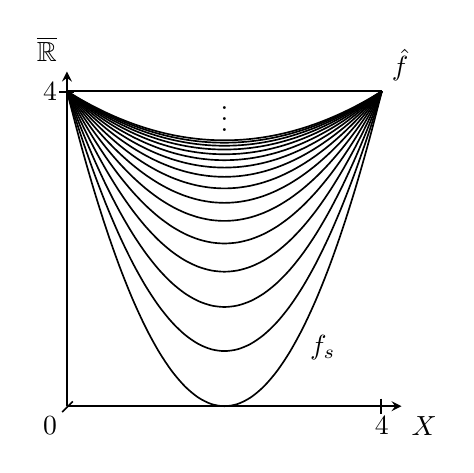
\begin{tikzpicture}[>=stealth, semithick]
            \node[below left] at (1, 0) {\(0\)};
            \draw[->] (1, 0) -- (1, 4.25) node[above left] {\(\overline{\mathbb{R}}\)};
            \node[left] at (1, 4) {\(4\)};
            \node[below] at (5, 0) {\(4\)};
            \draw[->] (1, 0) -- (5.25, 0) node[below right] {\(X\)};
            \node at (4.25, 0.75) {\(f_s\)};
            \draw[|-] (1, 4) -- (1, 3.999);
            \draw[|-] (5, 0) -- (4.999, 0);
            \draw[|-] (1, 0) -- (1.001, -0.001);
            \foreach \z in {1, 1.25, 1.25^2, 1.25^3, 1.25^4, 1.25^5, 1.25^6, 1.25^7, 1.25^8, 1.25^9, 1.25^10, 1.25^11, 1.25^12, 1.25^13, 1.25^14, 1.25^15} {
                % Lagrangian Interpolation
                \draw[domain=1:5, smooth] plot ({\x},  {(\x-3)*(\x-5)/2-(3.5-3.5*\z/1.25^15)*(\x-1)*(\x-5)/4+(\x-1)*(\x-3)/2});
            }
            \node at (3, 3.75) {\(\vdots\)};
            \draw[-] (1, 4) -- (5, 4) node[above right] {\(\hat{f}\)};
        \end{tikzpicture}
        \caption{Illustration of the proof argument for \Cref{supremum_convexity_lemma} by a sequence of parabolas. Consider for this case \(S = [0, 4] = X\) and for any \(s \in S\) the function \(f_s\) to be the parabola obtained by Lagrange Interpolation on the points \(\{(0, 4), (2, s), (4, 4)\}\).}
    \end{figure}

    \begin{theorem}[{\cite[pp. 201-204]{IoffeTihomirov}}] \label{supremum_theorem}
        Let \(S\) be a compact topological space and \(f\colon S \times X \to \overline{\mathbb{R}}\), s.t. for any \((s, x) \in S \times X\), \(f|_{\{s\} \times X}\) is convex and proper, and that \(f|_{S \times \{x\}}\) is upper semicontinuous, where we each omit the respective fixed argument. Let \(f_s \coloneqq f|_{\{s\} \times X}\) and set
        \begin{align}
            \hat{f}\colon X \to \overline{\mathbb{R}}, x \mapsto \sup_{s \in S} f_s(x) \text{ and } S_0\colon X \to \mathcal{P}(S), x \mapsto \{s \in S \mid f_s(x) = \hat{f}(x)\}.
        \end{align}
        In both of the following statements, the closures are taken wrt. the weak\({}^*\)-topology of \(X^*\).
        \begin{enumerate}[label=(\roman*), wide]
            \item \label{supremum_theorem_1} For any \(x \in X\)
            \begin{align}
                \overline{\text{conv}}\left(\bigcup_{s \in S_0(x)} \partial f_s(x)\right) \subseteq \partial \hat{f}(x)
            \end{align}
            \item \label{supremum_theorem_2} If for all \(s \in S\), \(f_s\) is continuous at a point \(x_0 \in X\), then
            \begin{align}
                \overline{\text{conv}}\left(\bigcup_{s \in S_0(x_0)} \partial f_s(x_0)\right) = \partial \hat{f}(x_0)
            \end{align}
        \end{enumerate}
    \end{theorem}

    \begin{figure}[!hbtp]
        \centering
        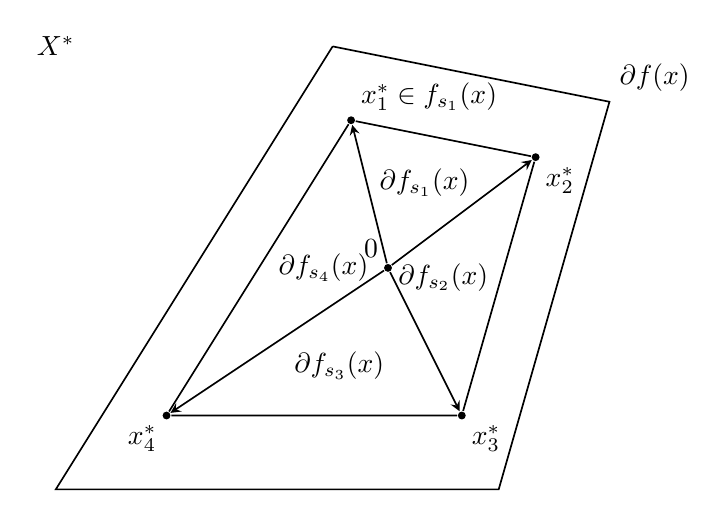
\begin{tikzpicture}[>=stealth, semithick, scale=0.75]
            \tikzset{
                point/.style={circle, fill, inner sep=0pt, minimum size=1mm}
            };
            \node at ($1.5*1.25*(-3, 0)+1.25*(0, 3)$) {\(X^*\)};
            \node[point] (0) at ($(0, 0)$) {};
            \node[point] (1) at ($1.25*(-0.5, 2)$) {};
            \node[point] (2) at ($1.25*(2, 1.5)$) {};
            \node[point] (3) at ($1.25*(1, -2)$) {};
            \node[point] (4) at ($1.25*(-3, -2)$) {};
            \node[above left] at (0) {\(0\)};
            \node[above right] at (1) {\(x_1^* \in f_{s_1}(x)\)};
            \node[below right] at (2) {\(x_2^*\)};
            \node[below right] at (3) {\(x_3^*\)};
            \node[below left] at (4) {\(x_4^*\)};
            \path[->]
                (0) edge (1)
                (0) edge (2)
                (0) edge (3)
                (0) edge (4)
            ;
            \node at ($(0) + 0.66*(1)!0.5!(2)$) {\(\partial f_{s_1}(x)\)};
            \node at ($(0) + 0.5*(2)!0.5!(3)$) {\(\partial f_{s_2}(x)\)};
            \node at ($(0) + 0.66*(3)!0.5!(4)$) {\(\partial f_{s_3}(x)\)};
            \node at ($(0) + 0.5*(4)!0.5!(1)$) {\(\partial f_{s_4}(x)\)};
            \draw (1) -- (2) -- (3) -- (4) -- (1);
            \draw ($1.5*(1)$) -- ($1.5*(2)$) -- ($1.5*(3)$) -- ($1.5*(4)$) -- ($1.5*(1)$);
            \node[above right] at ($1.5*(2)$) {\(\partial f(x)\)};
        \end{tikzpicture}
        \caption{Illustration of the statement in \Cref{supremum_theorem} on an example of a \(4\)-point space \(S\) and triangle-formed subdifferentials.}
    \end{figure}

    \begin{proof}
        \begin{enumerate}[label=(\roman*), wide]
            \item[\ref{supremum_theorem_1}] \draftcommentdone Apply \Cref{supremum_convexity_lemma} to \(\hat{f}\) to conclude its convexity. For \(x \in X\) and \(s \in S_0(x)\), we have \(f_s(x) = \hat{f}(x)\) and \(\partial f_s(x) \subseteq \partial \hat{f}(x)\), as for any \(x^* \in \partial f_s(x)\) and \(z \in X\)
            \begin{align}
                \hat{f}(x) + \langle x^*, z-x \rangle = f_s(x) + \langle x^*, z-x \rangle \leq f_s(z) \leq \hat{f}(z)
            \end{align}
            Since \(s\) was arbitrary, \(\bigcup_{s \in S_0(x)} \partial f_s(x) \subseteq \partial \hat{f}(x)\). Since \(\partial \hat{f}(x)\) is convex and weak\({}^*\)-closed \cite[p. 198]{IoffeTihomirov}, we have
            \begin{align}
                \overline{\text{conv}}\left(\bigcup_{s \in S_0(x)} \partial f_s(x)\right) \subseteq \partial \hat{f}(x)
            \end{align}
            which was the claim.
            \item[\ref{supremum_theorem_2}] \draftcommentdone Our overall strategy is a proof of equality by contradiction. We first prove the existence of a set-separating functional \ref{supremum_theorem_2_1}, then we use a separation theorem to obtain a point \(x \in X\) with a useful property \ref{supremum_theorem_2_2} and then we argue that we can wlog. assume \(\hat{f}(x_0 + x) < \infty\) \ref{supremum_theorem_2_3}. Lastly, we prove, that the first assumption violates the upper semicontinuity of \(f_{S \times \{x_0\}}\) \ref{supremum_theorem_2_4}.
            
            \begin{edgebox}
                \begin{theorem}[{\cite[pp. 164-165]{IoffeTihomirov}}] \label{separation_theorem}
                    Let \(A \subseteq X\) be closed, convex and let \(x \notin A\). Then there exists a functional \(x^* \in X^*\), s.t. \(\langle x^*, y\rangle \leq \langle x^*, x \rangle - \varepsilon\) for a fixed \(\varepsilon \in \mathbb{R}_{> 0}\) and any \(y \in A\), strongly separating \(A\) and \(\{x\}\).
                \end{theorem}
            \end{edgebox}

            \begin{enumerate}[label=(\alph*), wide]
                \item \label{supremum_theorem_2_1} \draftcommentdone Consider, that
                \begin{itemize}[wide]
                    \item for all \(s \in S\), \(\partial f_s(x_0) \neq \emptyset\) by \cite[p. 199]{IoffeTihomirov}, as the functions are continuous there, and
                    \item \(S_0(x_0) \neq \emptyset\), as by Weierstrass \cite[p. 13]{IoffeTihomirov}, \(f|_{S \times \{x_0\}}\) attains a maximum \(f_s(x_0)\) for some \(s \in S\).
                \end{itemize}
                The latter may not be true for any \(x \in X\), it is only true since every \(f_s\), \(s \in S\), is finite at \(x_0\). Set \(Q \coloneqq \overline{\text{conv}}(\bigcup_{s \in S_0(x_0)} \partial f_s(x_0))\). By the preceding argument we have \(Q \neq \emptyset\). Thus, we can suppose \(Q \neq \partial \hat{f}(x_0)\) and let \(x^* \in \partial \hat{f}(x_0) \setminus Q\).
                \item \label{supremum_theorem_2_2} \draftcommentdone \(Q\) is convex and closed, and \(x^* \notin Q\). \Cref{separation_theorem} gives the existence of some \(\hat{x} \in X^{**}\) and \(\varepsilon \in \mathbb{R}_{> 0}\), s.t. as discussed in the preliminaries in \Cref{preliminaries}, an \(x \in X\) fulfills
                \begin{align}
                    \hat{x}(x^*) = x^*(x) = \langle x^*, x \rangle \geq \sup_{z^* \in Q} \langle z^*, x\rangle + \varepsilon
                \end{align}
                \item \label{supremum_theorem_2_3} \draftcommentdone Note that scaling by a constant does not change the separation criterion for \(x\). So we may find such a constant. Since the functions \(f|_{\{s\} \times X}\) for a \(s \in S\) are continuous in \(x_0\), as well as proper and convex, they are especially finite there, and thus \(x_0 \in \text{dom}(\hat{f})\). The goal is first to prove that there is some \(\lambda \in \mathbb{R}_{> 0}\), s.t. \(\hat{f}(x_0+\lambda x) < \infty\), s.t. replacing \(x\) by \(\lambda x\) gives \(\hat{f}(x_0), \hat{f}(x_0+x) < \infty\).
                
                We proceed in a couple of steps. Let \(\varepsilon' \in \mathbb{R}_{> 0}\).
                \begin{itemize}[wide]
                    \item For every \(s \in S\), there is a \(\lambda_s \in \mathbb{R}_{> 0}\) with \(f_s(x_0+\lambda_s x) \leq f_s(x_0) + \varepsilon'\) by continuity of \(f_s\) and by the seminorm structure of locally convex TVS \cite[p. 426]{Werner}, more exactly by the fact that there is a null environment basis element that is circular.
                    \item Fix an \(s \in S\). \(f|_{S \times \{x_0+\lambda_s x\}}\) is upper semicontinuous, so there is an open neighborhood \(s \in U_s \subseteq S\) with \(f_{s'}(x_0+\lambda_s x) \leq f_s(x_0+\lambda_s x) + \varepsilon' \leq f_s(x_0) + 2\varepsilon'\) for any \(s' \in U_s\).
                    \item \(\{U_s\}_{s \in S}\) is thus an open cover of \(S\). By compactness, there are \(s_1, ..., s_m \in S\) for \(m \in \mathbb{N}_{\geq 1}\), s.t. \(\{U_{s_1}, ..., U_{s_m}\}\) covers \(S\). Choosing \(\lambda \coloneqq \min\{\lambda_{s_1}, ..., \lambda_{s_m}\} > 0\) gives \(f_s(x_0 + \lambda x) \leq \hat{f}(x_0)+2\varepsilon'\) for any \(s \in S\), which is the desired finiteness result.
                \end{itemize}
                Replace now for everything following, as announced, \(x\) with \(\lambda x\). As \(\hat{f}\) is convex, we can further directly conclude \(\hat{f}(x_0+tx) \leq (1-t)\hat{f}(x_0)+t\hat{f}(x_0+x) < \infty\) for any \(t \in [0, 1]\) by Jensens Inequality. In other words, \(x_0 + [0, 1] x \subseteq \text{dom}(\hat{f})\).
                \item \label{supremum_theorem_2_4} \draftcommentdone At last, we proceed with the main contradiction, which is again divided up into multiple steps.
                
                \begin{enumerate}[label=\arabic*., wide]
                    \item \label{supremum_theorem_2_4_1} We claim \(\lim_{t \to 0} \hat{f}(x_0+tx) = \hat{f}(x_0)\). \((\leq)\) Let \(s_0 \in S_0(x_0)\). We then have for any \(t \in [0, 1]\), that \(f_{s_0}(x_0+tx) \leq \hat{f}(x_0+tx)\). Taking the limit, as \(f|_{\{s_0\} \times X}\) is continuous in \(x_0\), gives \(\hat{f}(x_0) \leq \lim_{t \to 0} \hat{f}(x_0+tx)\). \((\geq)\) Use for a fixed \(t \in [0,1]\) Jensens Inequality to obtain \(\hat{f}(x_0+tx) \leq (1-t)\hat{f}(x_0)+t\hat{f}(x_0+x)\). Taking the limit gives \(\lim_{t \to 0} \hat{f}(x_0+tx) \leq \hat{f}(x_0)\). The sandwich rule of limit calculus now gives the statement.
                    \item Let \(t \in (0, 1)\) be fixed and choose \(s_t \in S\) with \(f_{s_t}(x_0+tx) = \hat{f}(x_0+tx)\). By Jensens inequality
                    \begin{align}
                        \hat{f}(x_0+tx) = f_{s_t}(x_0+tx) \leq (1-t)f_{s_t}(x_0)+tf_{s_t}(x_0+x)
                    \end{align}
                    Since \(f_{s_t}(x_0+x) \leq \hat{f}(x_0+x) < \infty\), we thus get
                    \begin{align}
                        \hat{f}(x_0+tx)-t\hat{f}(x_0+x) \leq (1-t)f_{s_t}(x_0)
                    \end{align}
                    Taking the limit \(t \to 0\) and using \(\lim_{t \to 0} \hat{f}(x_0+tx) = \hat{f}(x_0)\) from the argument in \ref{supremum_theorem_2_4_1}, as well as the product rule from limit calculus on the right side, we obtain \(\hat{f}(x_0) \leq \lim_{t \to 0} f_{s_t}(x_0)\). \(\lim_{t \to 0} f_{s_t}(x_0) \leq \hat{f}(x_0)\) follows directly by the monotonicity of limits. So \(\lim_{t \to 0} f_{s_t}(x_0) = \hat{f}(x_0)\) by the sandwhich rule of limit calculus.
                    \item \label{supremum_theorem_2_4_3} Let \(s_0 \in S\) be a cluster point of \(\{s_t\}_{t \in (0, 1)}\), which we recall exists, due to \(S\) being compact and \(\{s_t\}_{t \in (0, 1)}\) being infinite \cite[p. 12]{IoffeTihomirov}. \(f|_{S \times \{x_0\}}\) is upper semicontinuous, so consider for any \(\varepsilon'\) an open neighborhood \(U_{\varepsilon'} \subseteq S\) of \(S_0\) with \(f_{s}(x_0) \leq f_{s_0}(x_0) + \varepsilon'\) for any \(s \in U_{\varepsilon'}\). As \(s_0\) is a cluster point, there is some \(s_t\) with \(t \in [0, 1]\) with \(s_t \in U_{\varepsilon'}\). Using this fact now with any monotonically decreasing null sequence \((\varepsilon'_n \in \mathbb{R}_{\geq 0})_{n \in \mathbb{N}}\), we obtain \(\lim_{t \to 0} f_{s_t}(x_0) = \hat{f}(x_0) \leq f_{s_0}(x_0) \leq \hat{f}(x_0)\), where the latter inequality follows from the definitions. This gives the claimed equality by transitivity. Especially, \(s_0 \in S_0(x_0)\), so \(\partial f_{s_0}(x_0) \subseteq Q\).
                    \item We have the inequalities
                    \begin{align}
                        \frac{f_{s_t}(x_0+tx)-f_{s_t}(x_0)}{t} &\geq \frac{\hat{f}(x_0+tx)-\hat{f}(x_0)}{t}\\
                        &\geq \hat{f}'(x_0; x) \geq \langle x^*, x \rangle \geq \sup_{z^* \in \partial f_{s_0}(x_0) \subseteq Q} \langle z^*, x \rangle + \varepsilon = f'_{s_0}(x_0; x) + \varepsilon\\
                        &\leadsto f_{s_t}(x_0+tx) \geq f_{s_t}(x_0) + t(f_{s_0}'(x_0; x) + \varepsilon)
                    \end{align}
                    and
                    \begin{align}
                        \frac{f_{s_0}(x_0+t_1x)-f_{s_0}(x_0)}{t_1} \leq f'_{s_0}(x_0; x) + \frac{\varepsilon}{2}
                    \end{align}
                    with a sufficient choice of \(t_1\), using the limit in the definition of the directional derivative. For any \(t \in (0, t_1)\), we now have with Jensens Inequality
                    \begin{align}
                        \left(1-\frac{t}{t_1}\right) f_{s_t}(x_0) + \frac{t}{t_1} f_{s_t}(x_0+t_1x) &\geq f_{s_t}\left(\left(1-\frac{t}{t_1}\right)x_0+\frac{t}{t_1}(x_0+t_1x)\right)\\
                        &= f_{s_t}(x_0+tx) \geq f_{s_t}(x_0) + t(f_{s_0}'(x_0; x)+2 \cdot \varepsilon / 2)\\
                        &\geq f_{s_t}(x_0)+t\left(\frac{f_{s_0}(x_0+t_1x)-f_{s_0}(x_0)}{t_1}+\frac{\varepsilon}{2}\right)
                    \end{align}
                    Dividing both sides by \(t/t_1\) and reordering after \(f_{s_t}(x_0)\), we have
                    \begin{align}
                        f_{s_t}(x_0+t_1x) \geq f_{s_t}(x_0+t_1x) + \varepsilon t_1 / 2
                    \end{align}
                    Letting \(t \to 0\), we thus have with \ref{supremum_theorem_2_4_3}, where we observe that the argument can be repeated with \(x_0+t_1 x\) analogously, that
                    \begin{align}
                        \lim_{t \to 0} f_{s_t}(x_0+t_1x) \geq f_{s_0}(x_0+t_1x) + \varepsilon t_1/2
                    \end{align}
                    contradicting the upper semicontinuity of \(f|_{S \times \{x_0+t_1x\}}\) \lightning.
                    
                    
                    %By considering that \(\hat{f}\) is convex and proper and using the infimum rule for directional derivatives \cite[pp. 194-195]{IoffeTihomirov} and \ref{supremum_theorem_2_2}, we further have
                    %\begin{align}
                    %    \frac{\hat{f}(x_0+tx)-\hat{f}(x_0)}{t} \geq \hat{f}'(x_0; x) = \inf_{\lambda \in \mathbb{R}_{> 0}} \frac{\hat{f}(x_0+tx)-\hat{f}(x_0)}{\lambda} \geq \langle x^*, x \rangle \geq \sup_{z^* \in Q} \langle z^*, x \rangle + \varepsilon
                    %\end{align}
                \end{enumerate}
            \end{enumerate}
        \end{enumerate}
    \end{proof}

    \begin{remark}
        Some remarks about this version of the proof, especially in comparison with the book.
        \begin{enumerate}[label=(\roman*), wide]
            \item We have additionally assumed that \(f_s\) is proper for any \(s \in S\), as the use of \cite[p. 199]{IoffeTihomirov} requires that.
            \item In part \ref{supremum_theorem_2_3} of the proof, we defined \(U_s\) differently by taking neighborhoods directly from the definition of upper semicontinuity. In \cite[pp. 201-204]{IoffeTihomirov}, the sets \(\{s' \in S \mid f(s', x_0 + \lambda_s x) < \hat{f}(x_0) + 2\}\), claimed as being open, were used, leading to the same conclusion however.
            \item Further, the use of the partial subdifferential notation has been omitted here, instead \(f_s\) was used directly \cite[p. 47]{IoffeTihomirov}.
            \item As a personal note, the TVS \(X\) cannot have discrete topology, as the field is \(\mathbb{R}\) \cite[p. 426]{Werner}.
        \end{enumerate}
    \end{remark}

    \section{Situation in \(\mathbb{R}^n\) \draftcommentdone}

    Let \(n \in \mathbb{N}_{\geq 1}\) be fixed for the following.

    \phantom{}
    
    \textbf{Subdifferentiability in Finite Dimensions} We first consider the existence of subdifferentials in finite dimensions.

    \begin{lemma}[{\cite[p. 188]{IoffeTihomirov}}] \label{proper_convex_continuity_lemma}
        Let \(f\colon \mathbb{R}^n \to \overline{\mathbb{R}}\) be convex and proper.
        \begin{enumerate}[label=(\roman*), wide]
            \item \label{proper_convex_continuity_lemma_1} \(f\) is continuous with respect to \(\text{aff}({\text{dom}(f)})\) on \(\text{ri}(\text{dom}(f))\).
            \item \label{proper_convex_continuity_lemma_2} \(f^*\) is proper.
        \end{enumerate}
    \end{lemma}

    \begin{remark}
        Continuity with respect to a set is to be understood as treating the neighborhoods for continuity as subsets of the respected set. Recall especially, that we defined the relative interior as \cite[p. 44]{Rockafellar}
        \begin{align}
            \text{ri}(A) = \{a \in \text{aff}(A) \mid \, \exists \, \varepsilon \in \mathbb{R}_{> 0}\colon B(a, \varepsilon) \cap \text{aff}(A) \subseteq A\}
        \end{align}
        for some set \(A \subseteq \mathbb{R}^n\) and \(B(a, \varepsilon) = \{a' \in \mathbb{R}^n \mid \norm{a-a'}_{\ell_2} \leq \varepsilon\}\).
    \end{remark}

    \begin{figure}[!hbtp]
        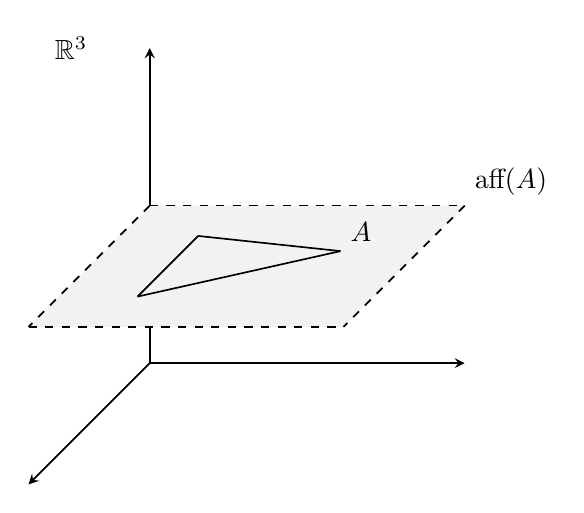
\begin{tikzpicture}[>=stealth, semithick]
            \node at (-1, 4, 0) {\(\mathbb{R}^3\)};
            \draw[->] (0, 0, 0) -- (4, 0, 0);
            \draw[->] (0, 0, 0) -- (0, 4, 0);
            \draw[->] (0, 0, 0) -- (0, 0, 4);
            \coordinate (a) at (1, 2, 1);
            \coordinate (b) at (3, 2, 1.5);
            \coordinate (c) at (1, 2, 3);
            \fill[gray!10] (0, 2, 0) -- (0, 2, 4) -- (4, 2, 4) -- (4, 2, 0);
            \draw (a) -- (c);
            \draw (a) -- (b);
            \draw (c) -- (b);
            \draw[dashed] (0, 2, 0) -- (0, 2, 4);
            \draw[dashed] (0, 2, 0) -- (4, 2, 0);
            \draw[dashed] (4, 2, 0) -- (4, 2, 4);
            \draw[dashed] (0, 2, 4) -- (4, 2, 4);
            \node[above right] at (b) {\(A\)};
            \node[above right] at (4, 2, 0) {\(\text{aff}(A)\)};
        \end{tikzpicture}
        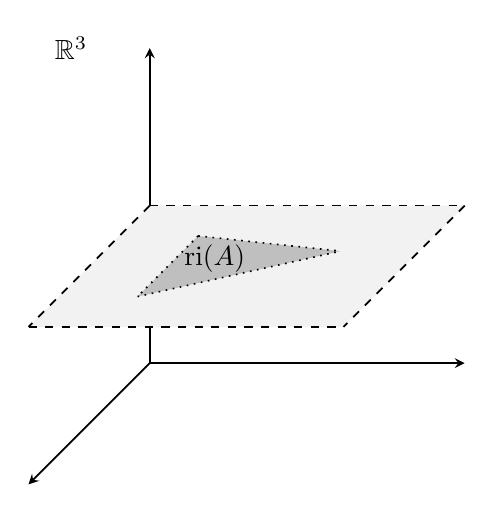
\begin{tikzpicture}[>=stealth, semithick]
            \node at (-1, 4, 0) {\(\mathbb{R}^3\)};
            \draw[->] (0, 0, 0) -- (4, 0, 0);
            \draw[->] (0, 0, 0) -- (0, 4, 0);
            \draw[->] (0, 0, 0) -- (0, 0, 4);
            \coordinate (a) at (1, 2, 1);
            \coordinate (b) at (3, 2, 1.5);
            \coordinate (c) at (1, 2, 3);
            \fill[gray!10] (0, 2, 0) -- (0, 2, 4) -- (4, 2, 4) -- (4, 2, 0);
            \fill[gray!50] (a) -- (b) -- (c);
            \draw[dotted] (a) -- (c);
            \draw[dotted] (a) -- (b);
            \draw[dotted] (c) -- (b);
            \draw[dashed] (0, 2, 0) -- (0, 2, 4);
            \draw[dashed] (0, 2, 0) -- (4, 2, 0);
            \draw[dashed] (4, 2, 0) -- (4, 2, 4);
            \draw[dashed] (0, 2, 4) -- (4, 2, 4);
            \node at (1.5, 2, 1.75) {\(\text{ri}(A)\)};
        \end{tikzpicture}
        \caption{Illustration of the concept of the relative interior.}
    \end{figure}

    \begin{theorem}[{\cite[p. 204]{IoffeTihomirov}}]
        Let \(f\colon \mathbb{R}^n \to \overline{\mathbb{R}}\) be proper and convex. Then \(f\) is subdifferentiable in \(\text{ri}(\text{dom}(f))\).
    \end{theorem}

    \begin{proof}
        \draftcommentdone Take \(x \in \text{ri}(\text{dom}(f))\). Consider the following chain of applications of proven theorems.
        \begin{enumerate}[wide]
            \item Since \(f\) is convex and proper, \Cref{proper_convex_continuity_lemma} \ref{proper_convex_continuity_lemma_1} gives the continuity at \(x\) with respect to \(\text{aff}(\text{dom}(f))\).
            \item \Cref{point_directional_derivative_continuity_theorem} \ref{point_directional_derivative_continuity_theorem_2} gives the finiteness of \(f'(x; \cdot)\) with respect to \(\text{aff}(\text{dom}(f))\).
            \item \(f'(x; \cdot)\) is convex and proper by that, so applying \Cref{proper_convex_continuity_lemma} \ref{proper_convex_continuity_lemma_1} again gives, that \(f'(x; \cdot)^*\) is proper.
            \item The effective domain of \(f'(x; \cdot)^*\) is the subdifferential \(\partial f'(x; 0) = \partial f(x)\) \cite[p. 196]{IoffeTihomirov}. Now, since \(f'(x; \cdot)^*\) is proper, \(\emptyset \neq \text{dom}(f'(x; \cdot)^*) = \partial f(x)\), concluding the proof.
        \end{enumerate}
    \end{proof}

    \begin{remark}
        In \cite[p. 172]{IoffeTihomirov}, it is stated that the supremum of the Young-Fenchel transform can only be taken for \(\text{dom}(f'(x; \cdot))\), which is false. Generally, taking it over \(f'(x; \cdot)^{-1}([0, \infty])\) suffices, which is \(\mathbb{R}^n\) for a proper \(f'(x; \cdot)\).
    \end{remark}
    
    \textbf{Representations of Subgradients in Finite Dimensions} The next main theorem will study representations of the functionals in subdifferentials.

    \begin{lemma}[{\cite[pp. 185-186]{IoffeTihomirov}}] \label{finite_dim_caratheodory_corollary}
        Let \(A \subseteq \mathbb{R}^n\) be bounded and closed. Then \(\text{conv}(A) = \overline{\text{conv}}(A)\).
    \end{lemma}

    \begin{lemma}[{\cite[p. 199]{IoffeTihomirov}}] \label{subdifferential_boundedness}
        For a proper convex function \(f\colon X \to \overline{\mathbb{R}}\), which is continuous at a point \(x_0\), \(\partial f(x_0)\) is non-empty, weakly\({}^*\) bounded and weakly\({}^*\) compact.
    \end{lemma}

    \begin{remark}
        Weakly\({}^*\) boundedness means that for a set \(A \subseteq X^*\) and any weak\({}^*\) neighborhood of zero \(U\) in \(X^*\), there is some \(\varepsilon \in \mathbb{R}_{> 0}\) with \(\varepsilon A \subseteq U\).
    \end{remark}

    \begin{lemma} \label{s_zero_s_zero_compact_lemma}
        Let \(X, S, f, f_s, \hat{f}, S_0, x_0\) be defined as in the setting of \Cref{supremum_theorem} \ref{supremum_theorem_2}. Then \(S_0(x_0)\) is compact.
    \end{lemma}

    \begin{proof}
        \draftcommentdone Since \(S\) is compact, it suffices to show that \(S_0(x_0)\) is closed \cite[p. 165]{Munkres}. Let \(s_* \in S\) be a cluster point of \(S_0(x_0)\). By upper semicontinuity, there is for any \(\varepsilon \in \mathbb{R}_{> 0}\) an open neighborhood \(s_* \in U_\varepsilon \subseteq S\), s.t. \(f_s(x_0) \leq f_{s_*}(x_0) + \varepsilon \, \forall \, s \in U_\varepsilon\). Since \(s_*\) is a cluster point of \(S_0(x_0)\), \(U_\varepsilon\) contains a point \(s' \in (U_\varepsilon \setminus \{s_*\}) \cap S_0(x_0)\). So \(\hat{f}(x_0) = f_{s'}(x_0) \leq f_{s_*}(x_0) + \varepsilon\). Since \(\varepsilon\) was chosen arbitrarily, \(\hat{f}(x_0) = f_{s_*}(x_0)\) and thus \(s_* \in S_0(x_0)\).
    \end{proof}

    \begin{figure}[!hbtp]
        \centering
        \begin{tikzpicture}[>=stealth, semithick]
            \draw (0, 0) -- (4, 0) node[below right] {\(X\)};
            \node at (0, 0) {\([\)};
            \node at (4, 0) {\(]\)};
            \node at (1, 0) {\((\)};
            \node at (3, 0) {\()\)};
            \draw[|->] (-0.25, 0) -- (-0.25, 4);
            \draw[|-] (-0.25, 3) -- (-0.25, 3);
            \draw[|-] (-0.25, 3.5) -- (-0.25, 3.5);
            \node[left] at (-0.25, 4) {\(\mathbb{R}\)};
            \node[left] at (-0.25, 0) {\(0\)};
            \node[left] at (-0.25, 3) {\(f_{s'}(x_0)\)};
            \node[left] at (-0.25, 3.5) {\(f_{s_*}(x_0)+\varepsilon\)};
            \node[below] at (1.5, 0) {\(s'\)};
            \draw[|-] (1.5, 0) -- (1.11, 0);
            \node[below] at (2, 0) {\(s_*\)};
            \draw[|-] (2, 0) -- (2.01, 0);
            \draw[|-] (1.5, 3) -- (1.5, 3.01);
            \node[rotate=-90] at (2, 3.5) {\([\)};
            \draw (2, 0) -- (2, 3.5);
            \node[below right] at (3, 0) {\(U_{\varepsilon}\)};
        \end{tikzpicture}
        \caption{Illustration of the argument of the proof of \Cref{s_zero_s_zero_compact_lemma} using for \(X\) a closed interval. Tightening both \(U_\varepsilon\) and the gap between \(f_{s_*}(x_0)+\varepsilon\) and \(f_{s'}(x_0)\), of which the latter is constant as \(\hat{f}(x_0)\), we obtain the statement.}
    \end{figure}

    \begin{remark}
        The proof of \Cref{s_zero_s_zero_compact_lemma} is due to Prof. Dr. Marita Thomas.
    \end{remark}

    \begin{theorem}[{\cite[pp. 204-205]{IoffeTihomirov}}] \label{finite_dim_representation_theorem}
        Let \(X, S, f, f_s, \hat{f}, S_0, x_0\) for \(X = \mathbb{R}^n\) and any \(s \in S\) be defined as in the setting of \Cref{supremum_theorem} \ref{supremum_theorem_2}. Then every \(y \in \partial \hat{f}(x_0)\) can be represented as a convex combination of form
        \begin{align}
            y = \sum_{i=1}^r \alpha_i y_i
        \end{align}
        with \(r \in \mathbb{N}\), \(1 \leq r \leq n+1\), \(\sum_{i=1}^r \alpha_i = 1\) and \(s_i \in S_0(x_0)\), \((\alpha_i, y_i) \in \mathbb{R}_{>0} \times \partial f_{s_i}(x_0)\) for any \(i \in \mathbb{N}\), \(1 \leq i \leq r\).
    \end{theorem}

    \begin{proof}
        The statement corresponds to the statement, that for \(P \coloneqq \bigcup_{s \in S_0(x_0)} \partial f_s(x_0)\), \(P\) is bounded and closed, because in that case \(\partial \hat{f}(x) = \overline{\text{conv}(P)} = \text{conv}(P)\) by \Cref{supremum_theorem} \ref{supremum_theorem_2} and \Cref{finite_dim_caratheodory_corollary}, since \((\mathbb{R}^n)^* \cong \mathbb{R}^n\). Because in that case, the convex combinations \(y = \sum_{i=1}^r \alpha_i y_i\) correspond exactly to all elements of \(\text{conv}(P)\). It only remains to show, that \(P\) is \ref{finite_dim_representation_theorem_1} bounded and \ref{finite_dim_representation_theorem_2} closed.

        \begin{enumerate}[label=(\alph*), wide]
            \item \label{finite_dim_representation_theorem_1} \draftcommentdone Using part \ref{supremum_theorem_2_3} of the proof of \Cref{supremum_theorem}, we find for any \(x \in X\) a \(\lambda \in \mathbb{R}_{> 0}\) with \(\hat{f}(x_0 + \lambda x) < \infty\). So \(\hat{f}'(x_0; \cdot)\) is finite, since \(\hat{f}'(x_0; x) = \inf_{\lambda' \in \mathbb{R}_{>0}} (\hat{f}(x_0+\lambda' x)-\hat{f}(x_0))/\lambda' \leq (\hat{f}(x_0+\lambda x)-\hat{f}(x_0))/\lambda < \infty\), where we also used, that \(\hat{f}\) is convex and proper. \(\hat{f}'(x_0; \cdot)\) is thus convex and proper and applying \Cref{proper_convex_continuity_lemma} \ref{proper_convex_continuity_lemma_1} gives, that it is continuous, as \(\text{dom}(f'(x_0; \cdot)) = \mathbb{R}^n\). By that, \(\hat{f}\) must be continuous in \(x_0\), as it would otherwise be unbounded in a neighborhood there and \(f'(x_0; \cdot)\) would thus not be continuous. \Cref{subdifferential_boundedness} gives the weakly\({}^*\) boundedness of \(\partial \hat{f}(x_0) \supseteq P\), thus also of \(P\).
            \item \label{finite_dim_representation_theorem_2} \draftcommentdone Let \((z_n \in P)_{n \in \mathbb{N}_{\geq 1}}\), s.t. \(z_n \to z \in \mathbb{R}^n\). Denote accordingly \(z_k \in \partial f_{s_k}(x_0)\) with \(s_k \in S_0(x_0)\) for every \(k \in \mathbb{N}_{\geq 1}\). As \(S_0(x_0)\) is compact by \Cref{s_zero_s_zero_compact_lemma}, \((s_k)_{k \in \mathbb{N}_{\geq 1}}\) has a cluster point \(s_0 \in S_0(x_0)\) by sequential compactness \cite[pp. 179-180]{Munkres}. With the upper semicontinuity of \(\hat{f}\), we thus have for any \(x \in \mathbb{R}^n\)
            \begin{align}
                f_{s_0}(x)-f_{s_0}(x_0) &\overset{\ref{finite_dim_representation_theorem_2_1}}{\geq} f_{s_0}(x)-\hat{f}(x_0) \overset{\ref{finite_dim_representation_theorem_2_2}}{\geq} \limsup_{k \to \infty} f_{s_k}(x) - \hat{f}(x_0)\\
                &\overset{\ref{finite_dim_representation_theorem_2_1}}{=} \limsup_{k \to \infty} f_{s_k}(x)-f_{s_k}(x_0) \geq \lim_{k \to \infty} \langle z_k, x-x_0 \rangle = \langle z, x-x_0 \rangle
            \end{align}
            \begin{enumerate}[label=(\arabic*), wide]
                \item \label{finite_dim_representation_theorem_2_1} \(\hat{f}(x_0) = f_{s_0}(x_0) = f_{s_k}(x_0)\) for any \(k \in \mathbb{N}_{\geq 1}\), as \(s_0, s_k \in S_0(x_0)\).
                \item \label{finite_dim_representation_theorem_2_2} Consider that \(s_0\) is a cluster point of \(\{s_k\}_{k \in \mathbb{N}_{\geq 1}}\) and the upper semicontinuity of \(f|_{\{s_0\} \times X}\), as in previous arguments.
            \end{enumerate}
            so \(z \in \partial f_{s_0}(x_0) \subseteq P\), concluding the statement.
        \end{enumerate}
    \end{proof}

    \begin{remark}
        The choices of \(r\) and the parameters \(\alpha_i\) stem from the use of \Cref{finite_dim_caratheodory_corollary}, a corollary of Carathéodory's Theorem.
    \end{remark}

    \printbibliography{}
\end{document}
